\documentclass[../../main/main.tex]{subfiles}
\graphicspath{{./figures/}}

\dominitoc
\faketableofcontents

\makeatletter
\renewcommand{\@chapapp}{M\'ecanique -- chapitre}
\makeatother

% \toggletrue{student}
% \HideSolutionstrue
% \toggletrue{corrige}
% \renewcommand{\mycol}{black}
\renewcommand{\mycol}{gray}

\begin{document}
\setcounter{chapter}{2}

\chapter{Mouvements courbes}

\vfill

\begin{prgm}
	\begin{tcb}*(ror)"know"{Savoirs}
		\begin{itemize}
			\item Identifier les degrés de liberté d'un mouvement. Choisir un système
			      de coordonnées adapté au problème.

			\item Systèmes de coordonnées cartésiennes, cylindriques et sphériques.

			\item Vitesse et accélération dans le repère de Frenet pour une
			      trajectoire plane.
		\end{itemize}
	\end{tcb}
	\begin{tcb}*(ror)"how"{Savoir-faire}
		\begin{itemize}
			\item Coordonnées cylindriques~: exprimer à partir d'un schéma le
			      déplacement élémentaire, construire le trièdre local associé et en
			      déduire géométriquement les composantes du vecteur vitesse.

			\item Établir les expressions des composantes des vecteurs position,
			      déplacement élémentaire, vitesse et accélération en coordonnées
			      cylindriques.

			\item Mouvement circulaire uniforme et non uniforme~: exprimer les
			      composantes du vecteur position, du vecteur vitesse et du vecteur
			      accélération en coordonnées polaires planes.

			\item Exploiter les liens entre les composantes du vecteur accélération,
			      la courbure de la trajectoire, la norme du vecteur vitesse et sa
			      variation temporelle.

			\item Établir l’équation du mouvement du pendule simple. Justifier
			      l’analogie avec l'oscillateur harmonique dans le cadre de
			      l'approximation linéaire.
		\end{itemize}
	\end{tcb}
\end{prgm}

\vfill

% \newpage

% \vspace*{\fill}
\vfill
\minitoc
\vfill
% \vspace*{\fill}

\newpage

% \tcblistof[\chapter*]{defi}{Liste des définitions}
% \tcblistof[\chapter*]{prop}{Liste des propriétés}

\chapter*{Liste des boîtes}
\tcblistof[\section*]{defi}{Définitions}

% \begin{tcb*}(defi)<lftt>{Mouvement plan}
% 	Un mouvement plan est dit \textbf{circulaire uniforme} s'il est à vitesse
% 	angulaire constante.
% \end{tcb*}
%
% \begin{center}
% 	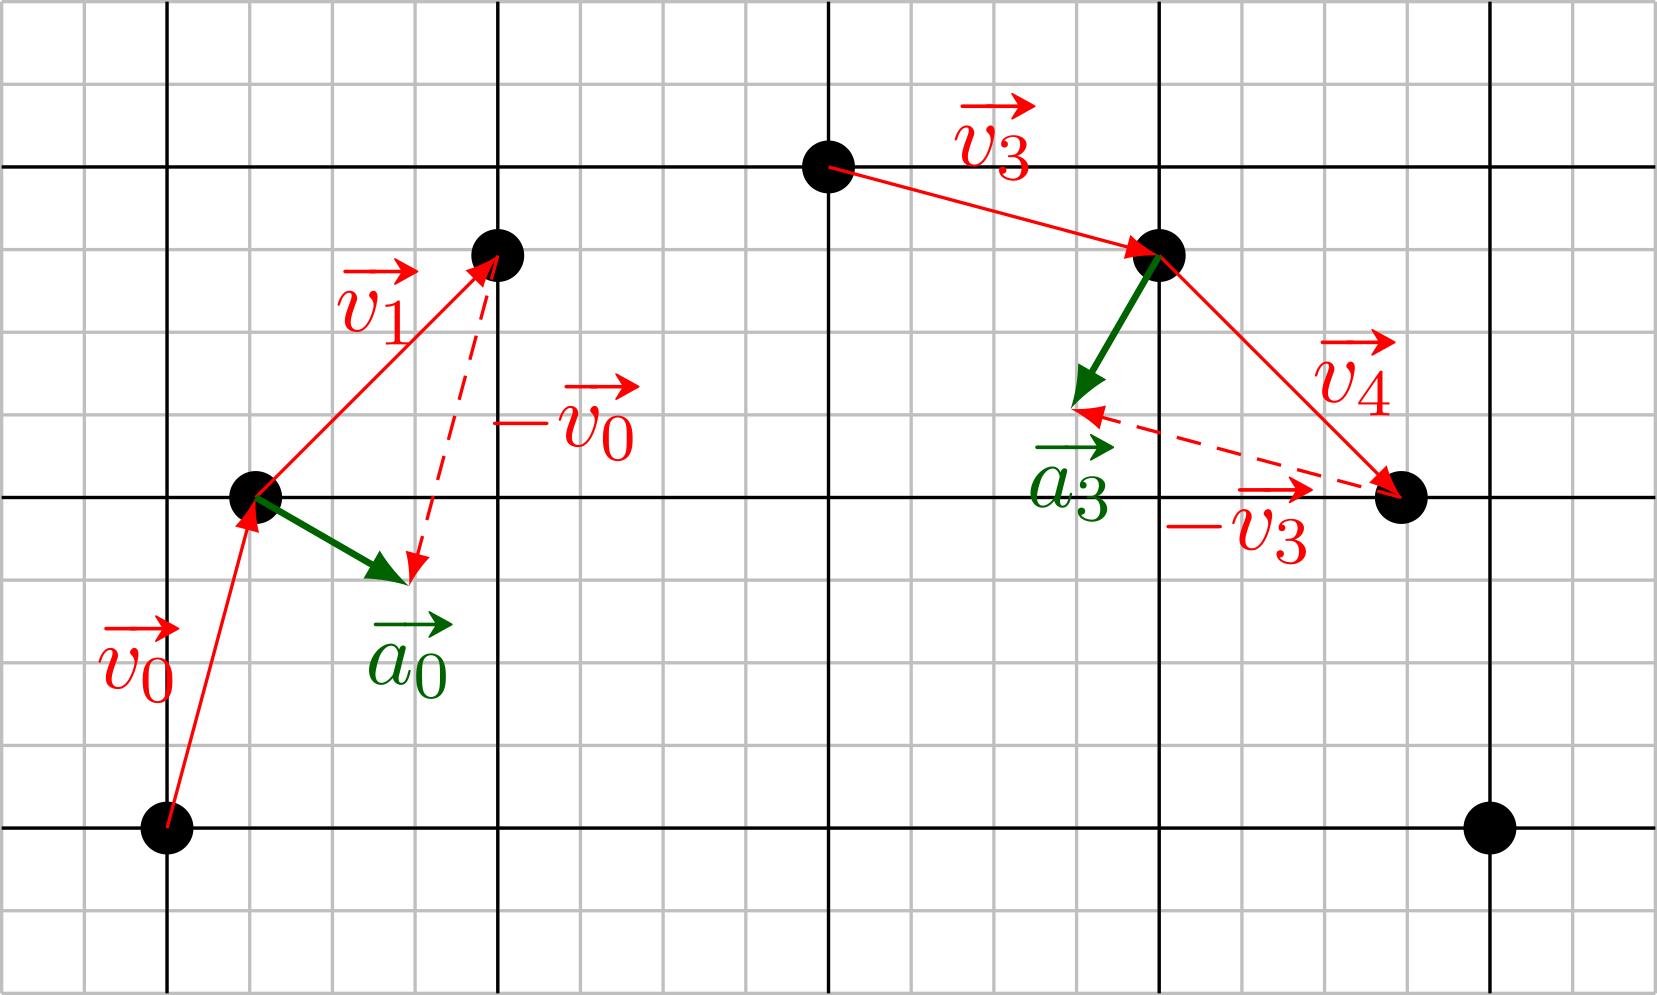
\includegraphics[width=.5\linewidth]{circ_va}
% \end{center}
%
% On observe sur cette figure que~: \bigbreak
% \begin{itemize}
% 	\item Le vecteur vitesse est de \underline{norme constante}, mais \textbf{sa
% 		      direction change} en étant \textbf{tangentielle à la trajectoire}~;
% 	\item Le vecteur accélération est de \underline{norme constante}, mais sa
% 	      \textbf{direction change} et \textbf{pointe vers le centre de rotation}.
% \end{itemize}
%
% \begin{tcb*}(ror){Direction vitesse et accélération}
% 	\centering
% 	Le vecteur vitesse est tangent à la trajectoire. Le vecteur accélération est
% 	toujours dirigé vers l’intérieur des courbes.
% \end{tcb*}
%
% Il ne paraît donc pas naturel d'utiliser les coordonnées cartésiennes dans ce
% cas-là.

\section{Mouvement courbe dans un plan}
\subsection{Position en coordonnées polaires}

\begin{tcb*}(defi){Repère polaire et vecteur position}
	\begin{minipage}{0.60\linewidth}
		Le repère polaire est constitué d'une origine O autour de laquelle sont
		définis deux vecteurs $\ur$ et $\ut$ de \textbf{direction
			variable dans le temps}, avec $\ur$ dans la direction $\OM$ et $\ut
			\perp \ur$ dans le sens direct tels que~:
		\[\boxed{\OM = r\ur}
			\qet
			\boxed{\norm{\OM} = r}\]
	\end{minipage}
	\hfill
	\begin{minipage}{0.35\linewidth}
		\begin{center}
			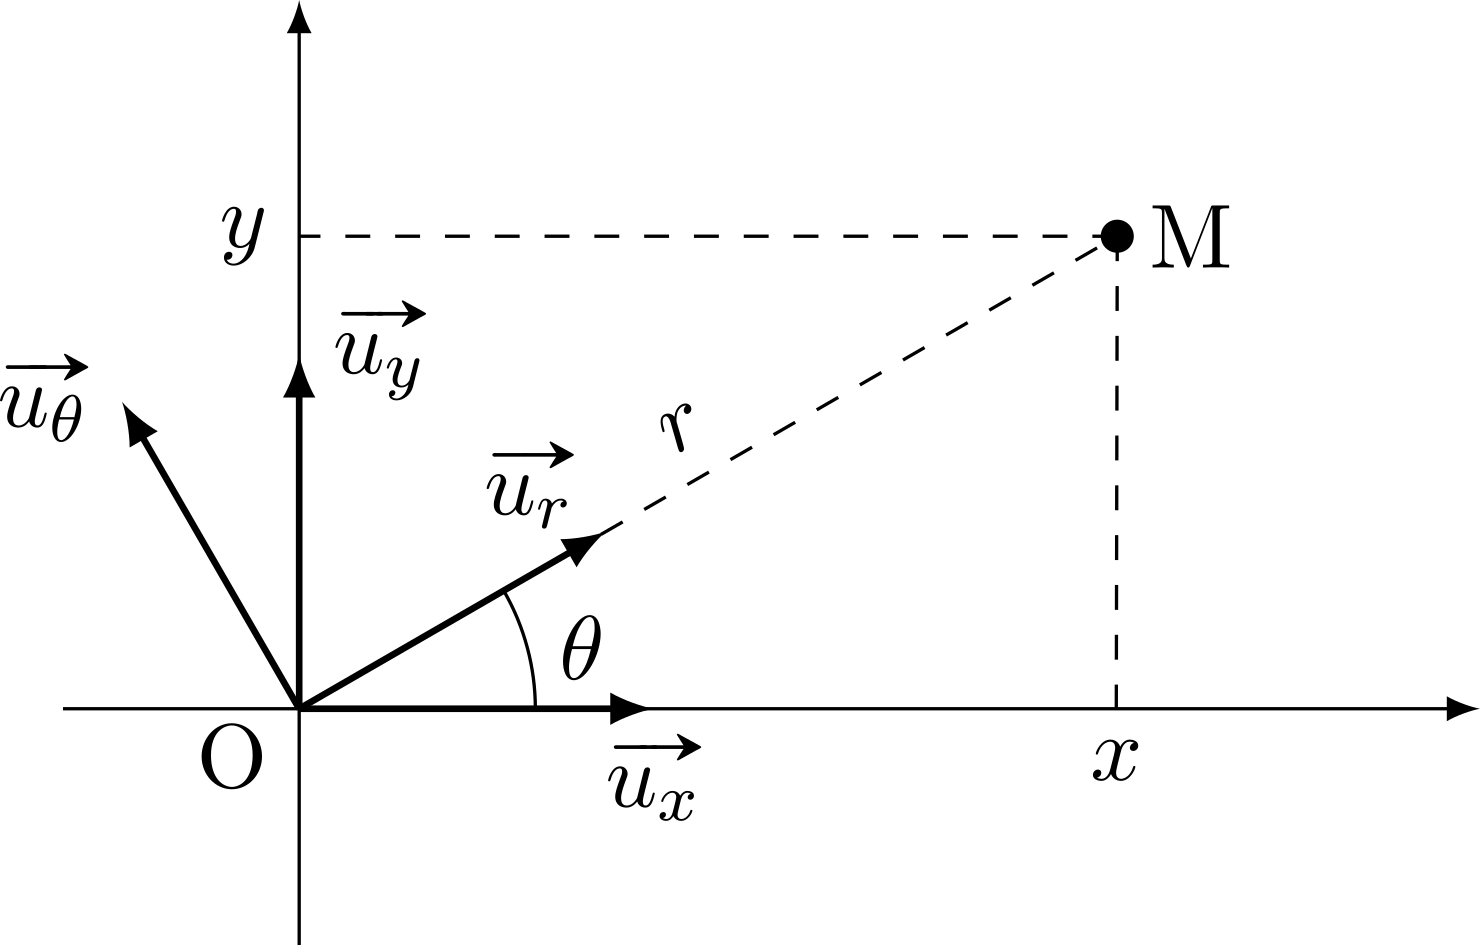
\includegraphics[width=\linewidth]{polaires}
		\end{center}
	\end{minipage}
\end{tcb*}

Soit un point matériel M dans l'espace~: il se repère en coordonnées
cartésiennes et polaires par
\[
	\OM = x\ux + y\uy
	\qet
	\OM = r\ur
	\qavec
	r = \sqrt{x^2+y^2} = \norm{\OM}
\]

On peut projeter les vecteurs de la base polaire sur la base cartésienne. Il
suffit pour cela de prendre des valeurs particulières de $\tt$, comme 0 et
$\pi/2$, pour trouver les dépendances en $\cos$ et $\sin$ suivantes~:
\[
	\ur = \cos(\tt)\ux + \sin(\tt)\uy
	\qet
	\ur = -\sin(\tt)\ux + \cos(\tt)\uy
\]

Ainsi, $r$, $\tt$ mais également $\ur$ et $\ut$ \textbf{dépendent du temps}.

\begin{tcb*}(prop){Position en polaires et projection cartésienne}
	En coordonnées polaires et dans le plan d'une trajectoire, le vecteur
	position s'écrit
	\[\boxed{\OM = r\ur}\]
	et les vecteurs $\ur$ et $\ut$ variables se décomposent sur $\ux$ et $\uy$
	fixes tels que
	\[
		\boxed{\ur = \cos(\tt)\ux + \sin(\tt)\uy}
		\qet
		\boxed{\ur = -\sin(\tt)\ux + \cos(\tt)\uy}
	\]
\end{tcb*}

\subsection{Vitesse en coordonnées polaires}
Par définition,
\begin{gather*}
	\vf = \dv{\OM}{t}
	\Lra
	\vf = \dv{r\ur}{t}
	\\\Lra
	\vf = \rp\ur + r\dv{\ur}{t}
\end{gather*}
Pour déterminer la vitesse il faut donc déterminer la variation dans le temps du
vecteur $\ur$.

\begin{tcb*}(demo)<lftt>{Vitesse en polaires}
	Pour cela, on décompose $\ur$ dans la base cartésienne qui, elle, a des
	vecteurs de base fixes dans le temps~:
	\begin{align*}
		\ur                 & = \cos(\tt)\ux + \sin(\tt)\uy
		\\\Lra
		\dv{\ur}{t}         & = \dv{\cos(\tt)}{t}\ux + \dv{\sin(\tt)}{t}\uy
		\\\Lra
		\dv{\ur}{t}         & = -\tp\sin(\tt)\ux + \tp\cos(\tt)\uy
		\\\Lra
		\dv{\ur}{t}         & = \tp
		\underbrace{\left(-\sin(\tt)\ux + \cos(\tt)\uy\right)}_{= \ut}
		\\\Lra
		\Aboxed{\dv{\ur}{t} & = \tp\ut}
	\end{align*}
\end{tcb*}

\begin{tcb*}(prop){Vitesse en coordonnées polaires}
	Ainsi, la vitesse en coordonnées polaires s'écrit
	\[\boxed{\vf = \rp\ur + r\tp\ut}\]
\end{tcb*}

\subsection{Déplacement élémentaire en polaires}
On a toujours $\dd\OM = \OM(t+\dt) - \OM(t)$, autrement dit $\dd\OM = \vf\dt$.
Ainsi, il suffit de prendre l'expression de la vitesse et de simplifier les
$\dt$ des dérivées temporelles~; on a donc
\begin{gather*}
	\dd\OM = \left(\frac{\dd{r}}{\cancel{\dt}}\ur + r
	\frac{\dd{\tt}}{\cancel{\dt}}\ut\right)\times\cancel{\dt}
\end{gather*}

\begin{tcb*}(prop){Déplacement élémentaire polaire}
	\begin{minipage}{0.70\linewidth}
		En coordonnées polaires, le déplacement élémentaire s'exprime
		\[\boxed{\dd\OM = \dd r\ur + r\dd\tt\ut}\]
	\end{minipage}
	\hfill
	\begin{minipage}{0.25\linewidth}
		\begin{center}
			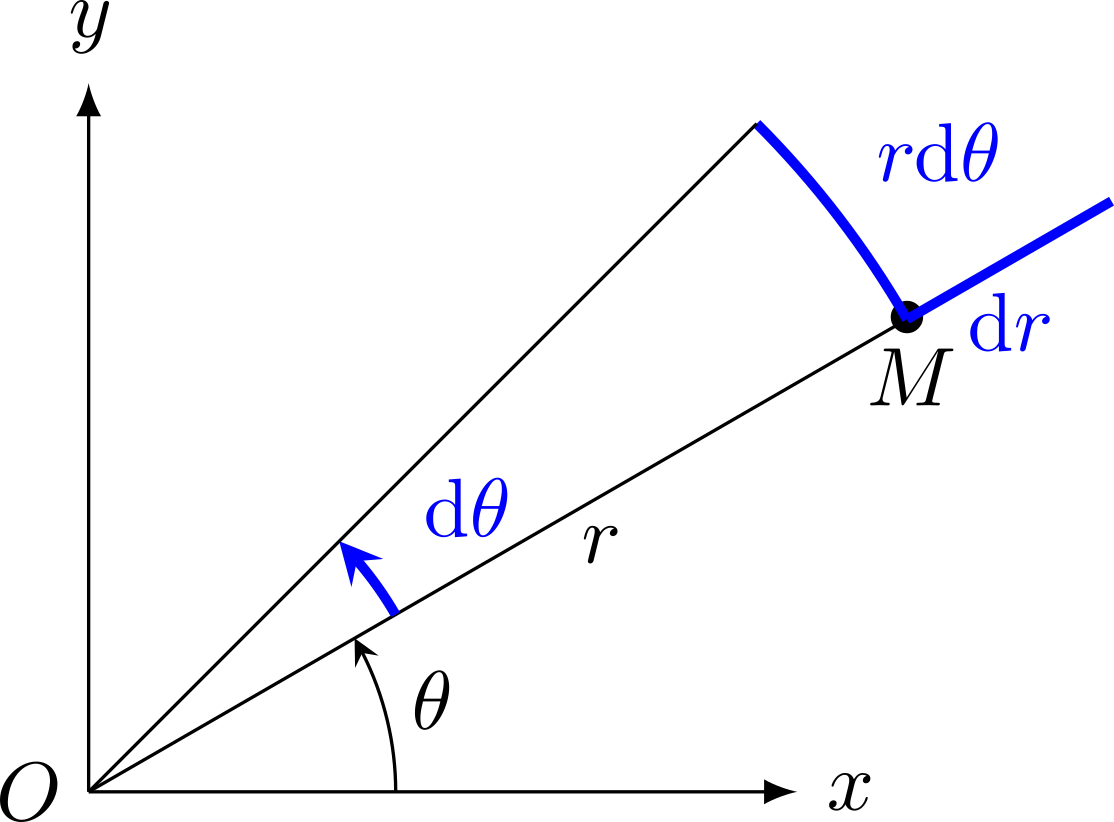
\includegraphics[width=\linewidth]{pol_dom}
		\end{center}
	\end{minipage}
\end{tcb*}

\subsection{Accélération}
On procède de la même façon que pour la vitesse~:
\begin{gather*}
	\af = \dv{\vf}{t}
	\Lra
	\af = \dv{\left(\rp\ur + r\tp\ut\right)}{t}
	\\\Lra
	\af = \rpp\ur + \rp \dv{\ur}{t} + \rp\tp\ut + r\tpp\ut + r\tp \dv{\ut}{t}
\end{gather*}
Pour déterminer l'accélération, il faut donc déterminer la variation dans le
temps du vecteur $\ut$.

\begin{tcb*}(demo)<lftt>{Dérivée de $\protect\ut$}
	Pour cela, on décompose $\ut$ dans la base cartésienne qui a des
	vecteurs de base fixes dans le temps~:
	\begin{align*}
		\ut                 & = -\sin(\tt)\ux + \cos(\tt)\uy
		\\\Lra
		\dv{\ut}{t}         & = \dv{-\sin(\tt)}{t}\ux + \dv{\cos(\tt)}{t}\uy
		\\\Lra
		\dv{\ut}{t}         & = -\tp\cos(\tt)\ux - \tp\sin(\tt)\uy
		\\\Lra
		\dv{\ut}{t}         & = -\tp
		\underbrace{\left(\cos(\tt)\ux + \sin(\tt)\uy\right)}_{= \ur}
		\\\Lra
		\Aboxed{\dv{\ut}{t} & = -\tp\ur}
	\end{align*}
\end{tcb*}

\leftcenters{Ainsi,}{$\af = \rpp\ur + \rp\tp\ut + \rp\tp\ut+r\tpp\ut -
		r\tp^2\ur$}

\begin{tcb*}(prop){Accélération en coordonnées polaires}
	Finalement, la vitesse en coordonnées polaires s'écrit
	\[\boxed{\af = \left( \rpp -r\tp^2 \right)\ur + \left( 2\rp\tp+r\tpp
			\right)\ut}\]
\end{tcb*}

\section{Exemples de mouvements plans}
\subsection{Mouvement circulaire}

\begin{tcb*}(defi)<lftt>{Mouvement circulaire}
	Un mouvement est dit \textbf{circulaire} s'il se fait dans un plan, à une
	distance de l'axe de rotation $r$ constante, soit
	\[
		r(t) = R
	\]
\end{tcb*}

Dans ce cas-là, on a
\[
	\OM = r(t)\ur = R\ur
	\qavec
	\rp = 0 = \rpp
\]

En notant $\w = \tp$ la vitesse angulaire, la vitesse et l'accélération donnent
\[
	\vf = R\w\ut
	\qet
	\af = -R\w^2\ur + R\wp\ut
\]

\subsection{Mouvement circulaire uniforme}
\begin{tcb*}(defi)<lftt>{Mouvement circulaire uniforme}
	Un mouvement est dit \textbf{circulaire \textit{uniforme}} si c'est un
	mouvement circulaire ($r(t) = \cte$) à \textit{vitesse angulaire
		constante}, soit
	\[
		\left\{
		\begin{array}{rcl}
			r(t)   & = & R  \\
			\tp(t) & = & \w
		\end{array}
		\right.
	\]
\end{tcb*}

Dans ce cas, $\rp = 0 = \rpp$ mais également $\tpp = 0$, donc la vitesse et
l'accélération donnent
\[
	\vf = R\w\ut
	\qet
	\af = -R\w^2\ur
\]

\begin{tcb*}(ror){Observations mouvement circulaire}
	Dans le cas du mouvement circulaire uniforme,
	\begin{itemize}
		\item Le vecteur vitesse est selon $\ut$ et est de norme constante,
		      égale à $R\w$~;
		\item Le vecteur accélération pointe vers le centre et est de norme
		      constance, égale à $\DS R\w^2 = \frac{v^2}{R}$.
	\end{itemize}
\end{tcb*}

\begin{tcb}*(expe)<itc>"trans"{Transition}
	Si la trajectoire d'un objet change de courbure, il peut être fastidieux de
	travailler avec les coordonnées polaires~: on utilisera alors un repère
	attaché à l'objet.
\end{tcb}

\subsection{Repère de \textsc{Frenet}}

\begin{tcb*}(defi){Repère de \textsc{Frenet}}
	\begin{minipage}{0.70\linewidth}
		Pour un point M sur une trajectoire courbe, on peut approximer la
		trajectoire à un instant $t$ comme étant celle d'un cercle, appelé
		\textbf{cercle osculateur}, localement tangent à la trajectoire et de rayon
		$R$. On définit alors le repère de \textsc{Frenet} avec~: \bigbreak
		\begin{itemize}
			\item $\vv{u_T}$ tangent à la trajectoire en M~;
			\item $\vv{u_N} \perp \vv{u_T}$ et dirigé vers l'intérieur de la
			      courbe, vers le centre du cercle osculateur.
		\end{itemize}
	\end{minipage}
	\hfill
	\begin{minipage}{0.25\linewidth}
		\begin{center}
			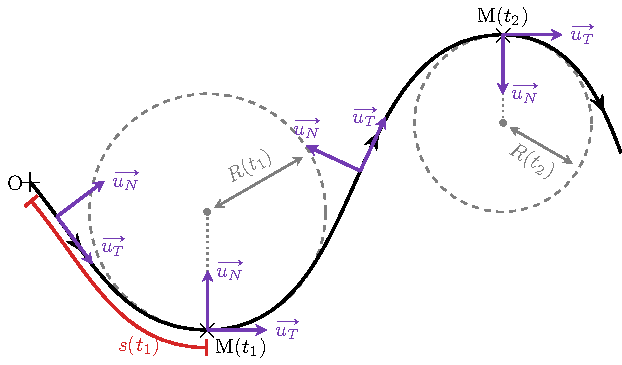
\includegraphics[width=\linewidth]{frenet}
		\end{center}
	\end{minipage} \bigbreak
	Le rayon $R$ est appelé \textbf{rayon de courbure}, et son inverse $\gamma =
		1/R$ est appelé \textbf{courbure} de la trajectoire.
\end{tcb*}

On peut alors exprimer la vitesse et l'accélération dans ce repère~; pour la
vitesse, on repart de la définition~:
\begin{gather*}
	\vf
	= \dv{\OM(t+\dt)-\OM(t)}{t}
	= \dv{\OM(t+\dt)+\vec{\Mr(t)\Or}}{t}
	= \dv{\vec{\Mr(t)\Mr(t+\dt)}}{t}
\end{gather*}
Or, par définition, la trajectoire est l'ensemble des positions du point M dans
le temps, donc le vecteur $\vec{\Mr(t)\Mr(t+\dt)}$ défini la trajectoire et la
direction du vecteur $\vv{u_T}$~; ainsi, \textbf{la vitesse est tangente à la
	trajectoire} et on a
\[
	\boxed{\vf = v\vv{u_T}}
\]

Concernant l'accélération, avec la définition du rayon de courbure on admet
\[ \dv{\vv{u_T}}{t} = \frac{v}{R}\vv{u_N}\]
et ainsi
\[
	\boxed{\af = \dv{v}{t}\vv{u_T} + \frac{v^2}{R}\vv{u_N}}
\]

\begin{itemize}
	\item On retrouve le mouvement rectiligne uniforme avec $R = +\infty \Lra
		      \gamma = 0$, puisqu'on a alors
	      \[\af = \dv{v}{t}\vv{u_T}\]
	      avec $\vv{u_T}$ dans le sens de la trajectoire.

	\item On retrouve également le mouvement circulaire puisque dans ce cas la
	      trajectoire \textbf{est} le cercle osculateur, donc $\vv{u_T} = \ut$ et
	      $\vv{u_N} = -\ur$.
\end{itemize}

\section{Application~: pendule simple}

\subsection{Tension d'un fil}
\begin{tcb*}(defi){Tension d'un fil}
	Un point matériel M accroché à un fil tendu subit de la part de ce fil une
	force appelée \textbf{tension du fil} et notée $\Tf$ telle que
	\[\boxed{\Tf = \norm{\Tf}\uf_{\Mr\ra\rm fil}}\]
	avec $\uf_{\Mr\ra\rm fil}$ un vecteur unitaire dirigé du point M vers le fil
	et $\norm{\Tf}$ la norme de la tension du fil. La \textbf{condition de
		tension} du fil est $\norm{\Tf} > 0$.

	\begin{minipage}{0.45\linewidth}
		\begin{center}
			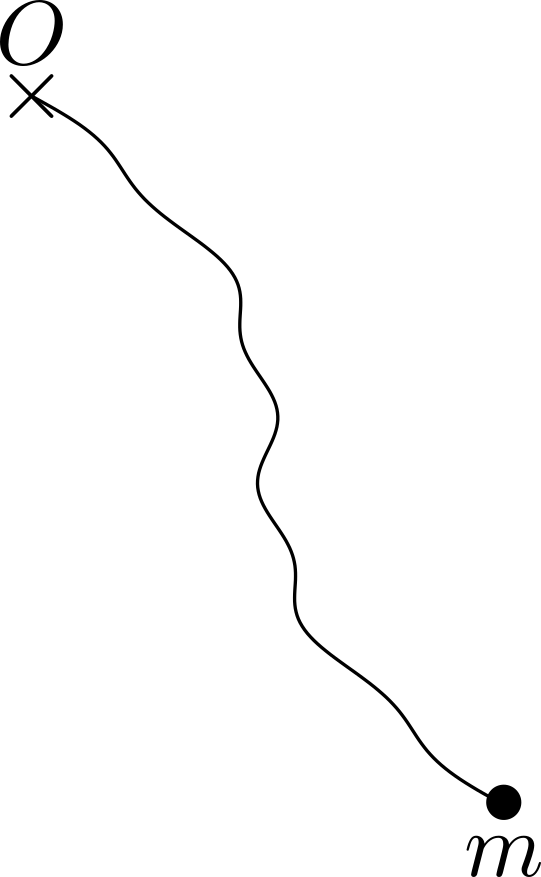
\includegraphics[height=3cm]{tension_null}
			\captionof{figure}{Fil détendu~: pas de force.}
		\end{center}
	\end{minipage}
	\hfill
	\begin{minipage}{0.45\linewidth}
		\begin{center}
			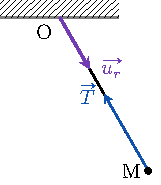
\includegraphics[height=3cm]{tension}%
			\captionof{figure}{Fil tendu~: force vers O.}%
		\end{center}
	\end{minipage}
\end{tcb*}

\subsection{Pendule simple}
Et si je vous disais qu'on peut mesurer l'attraction de la pesanteur… avec un
bout de ficelle et une masse~?
\bigbreak

\hspace*{-0.75cm}
\begin{minipage}{0.70\linewidth}
	\begin{enumerate}[label=\sqenumi]
		\bitem{De quoi parle-t-on~?} On étudie le mouvement d'une masse de
		\SI{20}{g} suspendue à un fil, dans le référentiel du laboratoire
		supposé galiléen. La masse est écartée de sa position d'équilibre et
		lâchée sans vitesse initiale.
		\bitem{Schéma}.
		\bitem{Modélisation.} On choisit d'utiliser des coordonnées polaires.
		\begin{itemize}
			\item La masse est assimilée à un point matériel M.
			\item Origine~: point d'accroche du fil (centre de rotation
			      pendule).
			\item Repère~: $(O,\ur,\ut)$ avec base polaire (voir schéma).
			\item $t$ initial~: moment du lâché, $\tt(0) = \tt_0$ et
			      $\tt(0) = 0$.
		\end{itemize}
	\end{enumerate}
\end{minipage}
\hfill
\begin{minipage}{0.25\linewidth}
	\begin{center}
		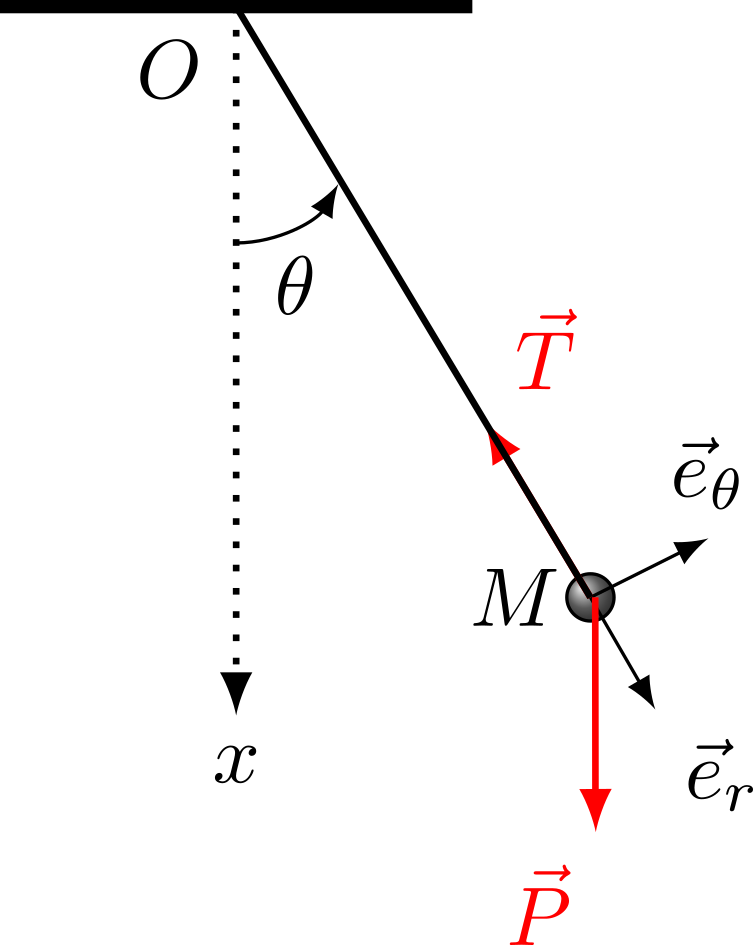
\includegraphics[width=\linewidth]{pendule_plain}
	\end{center}
\end{minipage}
\begin{enumerate}[label=\sqenumi, start=4]
	\bitem{Bilan des forces.}
	\[
		\begin{array}{ll}
			\textbf{Poids}   & \Pf = m\gf = mg(\cos\tt \ur - \sin\tt \ut) \\
			\textbf{Tension} & \Tf = -T\ur
		\end{array}
	\]
	\bitem{PFD.}
	\[m\af = \Pf + \Tf\]
	Le mouvement étant circulaire (mais pas uniforme), on a
	\[\af = -\ell\tp^2 \ur + \ell\tpp \ut\]
	\bitem{Équations scalaires.} On projette le PFD sur les axes~:
	\[
		\left\{
		\begin{array}{rcl}
			-m\ell\tp^2 & = & mg\cos\tt - T \\
			m\ell\tpp   & = & -mg\sin\tt
		\end{array}
		\right.
	\]
	\bitem{Résolution.} La première équation n'est pas utilisable telle qu'elle,
	puisque $T$ n'est pas connue~; cependant la seconde donne une équation
	différentielle homogène~:
	\[\boxed{\tpp + \frac{g}{\ell}\sin\tt = 0}\]
	qui constitue l'équation du mouvement du pendule. Sous cette forme, elle
	est \textbf{non-linéaire} donc non résoluble analytiquement~; elle peut
	l'être numériquement, voir
	\texttt{Capytale}\footnote{\url{
			https://capytale2.ac-paris.fr/web/c/a7c5-1241282}}.
\end{enumerate}
En revanche, dans l'approximation des petits angles, on a $\sin\tt\approx\tt$,
et ainsi on obtient~:
\[\boxed{\tpp + \frac{g}{\ell}\tt = 0}\]
\textbf{C'est l'équation différentielle d'un oscillateur harmonique~!} On met
donc en évidence la pulsation propre
\[\w_0 = \sqrt{\frac{g}{\ell}}\]
et on a la solution générale homogène~:
\[\tt(t) = A\cos(\w_0t) + B\sin(\w_0t)\]
On obtient $A$ et $B$ avec les CI,
\begin{gather*}
	\tt(0) = \tt_0
	\Lra A\times 1 + B\times 0 = \tt_0
	\qdonc
	\boxed{A = \tt_0}\\
	\tp(0) = 0
	\Lra -A\w_0\times 0 + B\w_0\times 1 = 0
	\qdonc
	\boxed{B = 0}
\end{gather*}
\leftcenters{et finalement}{$\boxed{\tt(t) = \tt_0\cos(\w_0t)}$}

Le pendule oscille à la pulsation $\w_0$ et à la période $T_0$ telles que
\[
	\w_0 = \sqrt{\frac{g}{\ell}}
	\qet
	T_0 = 2\pi \sqrt{\frac{\ell}{g}}
	\qdonc
	\boxed{g = \frac{4\pi^2\ell}{T_0{}^2}}
\]

Dans cette approximation, la période ne dépend ni de la masse, ni de l'angle
initial. En réalité, si on s'écarte beaucoup de la verticale ($\abs{\theta} >
	\pi/4$), la période change et n'est plus celle que l'on a aux petits angles.
Voir le changement sur le graphique ci-dessous et en
ligne\footnote{\url{http://www.sciences.univ-nantes.fr/sites/genevieve_tulloue/Meca/Oscillateurs/periode_pendule.php}}.

\begin{minipage}{0.45\linewidth}
	\begin{center}
		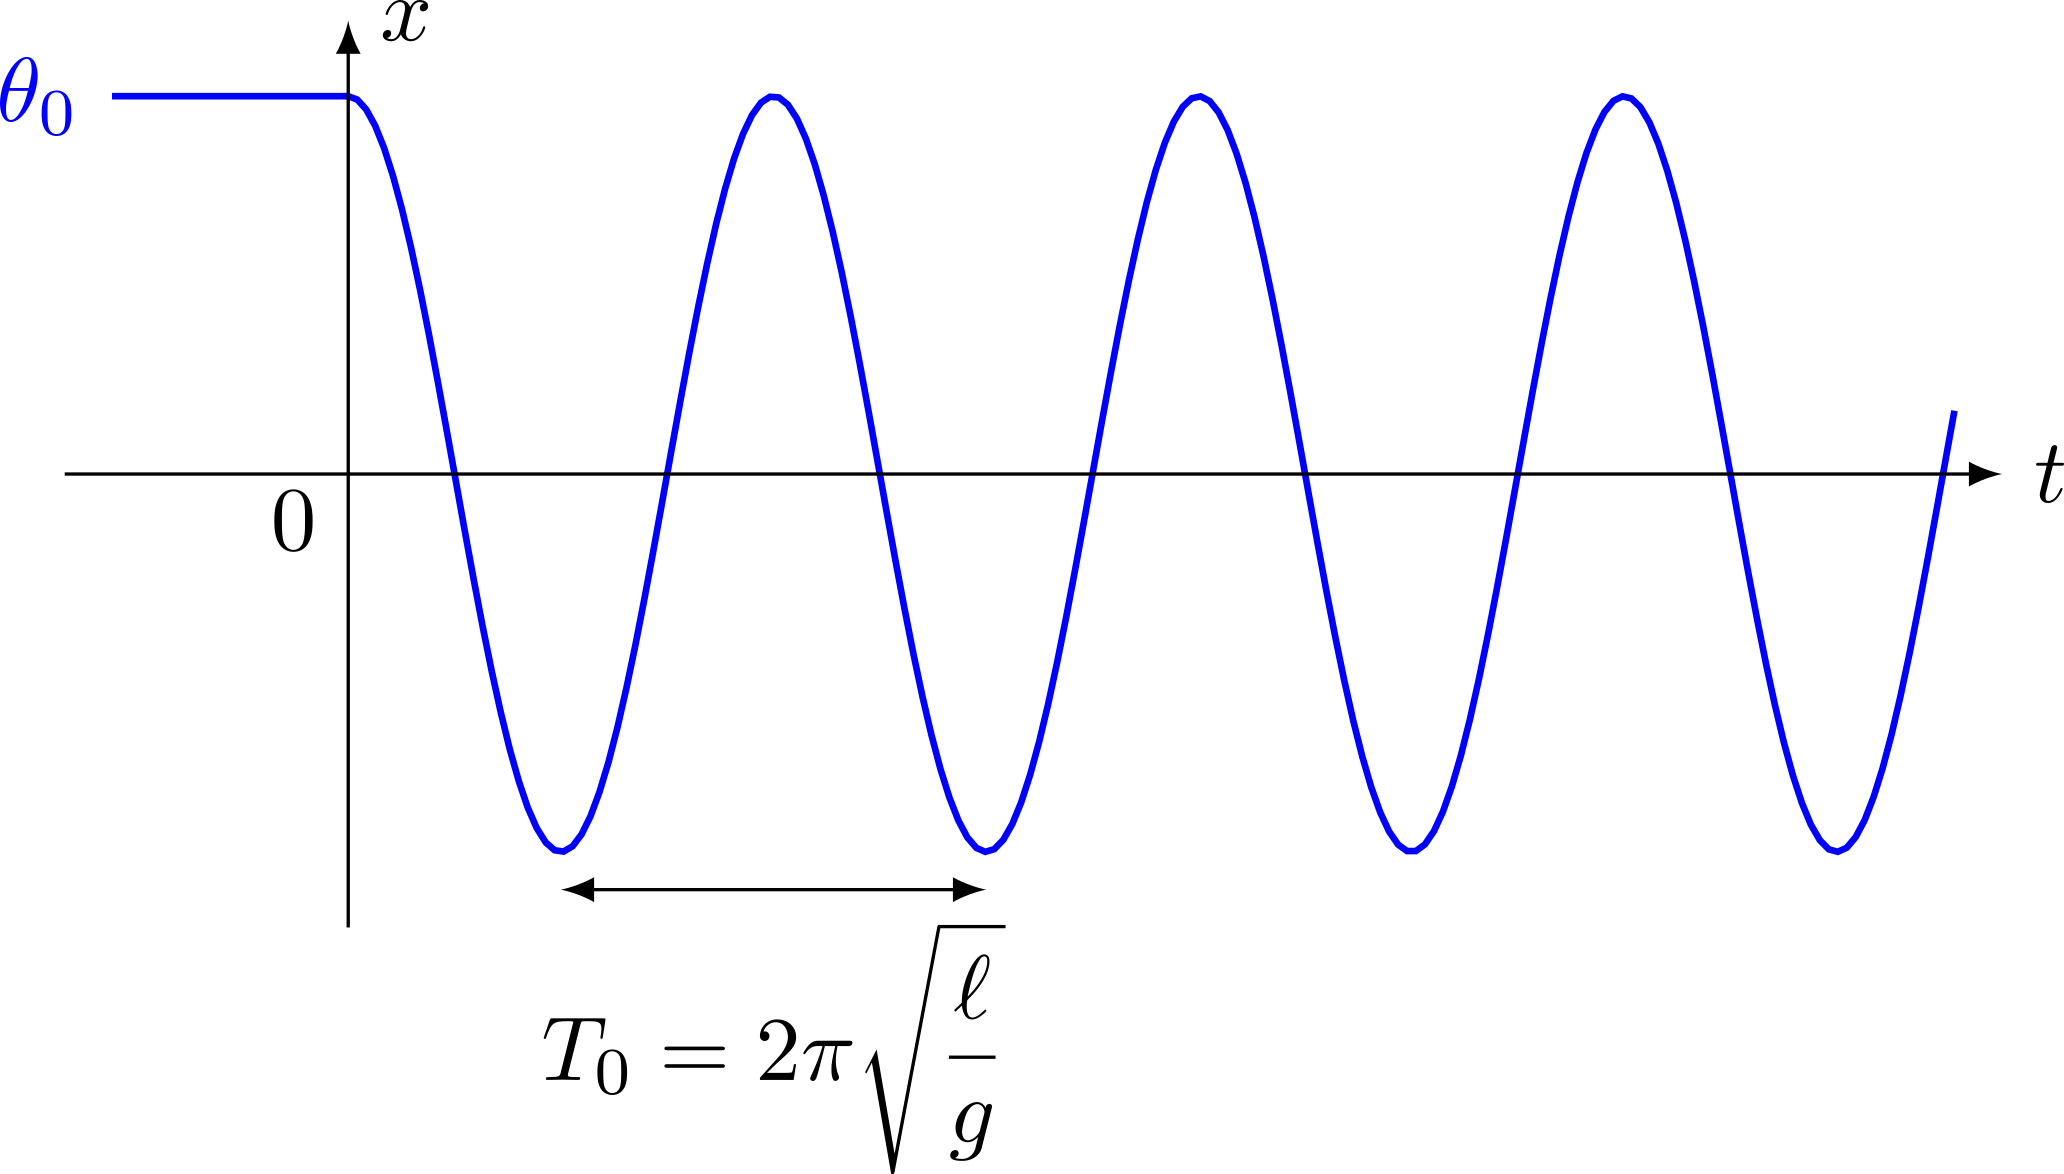
\includegraphics[width=\linewidth]{pendule_sol}
	\end{center}
\end{minipage}
\hfill
\begin{minipage}{0.45\linewidth}
	\begin{center}
		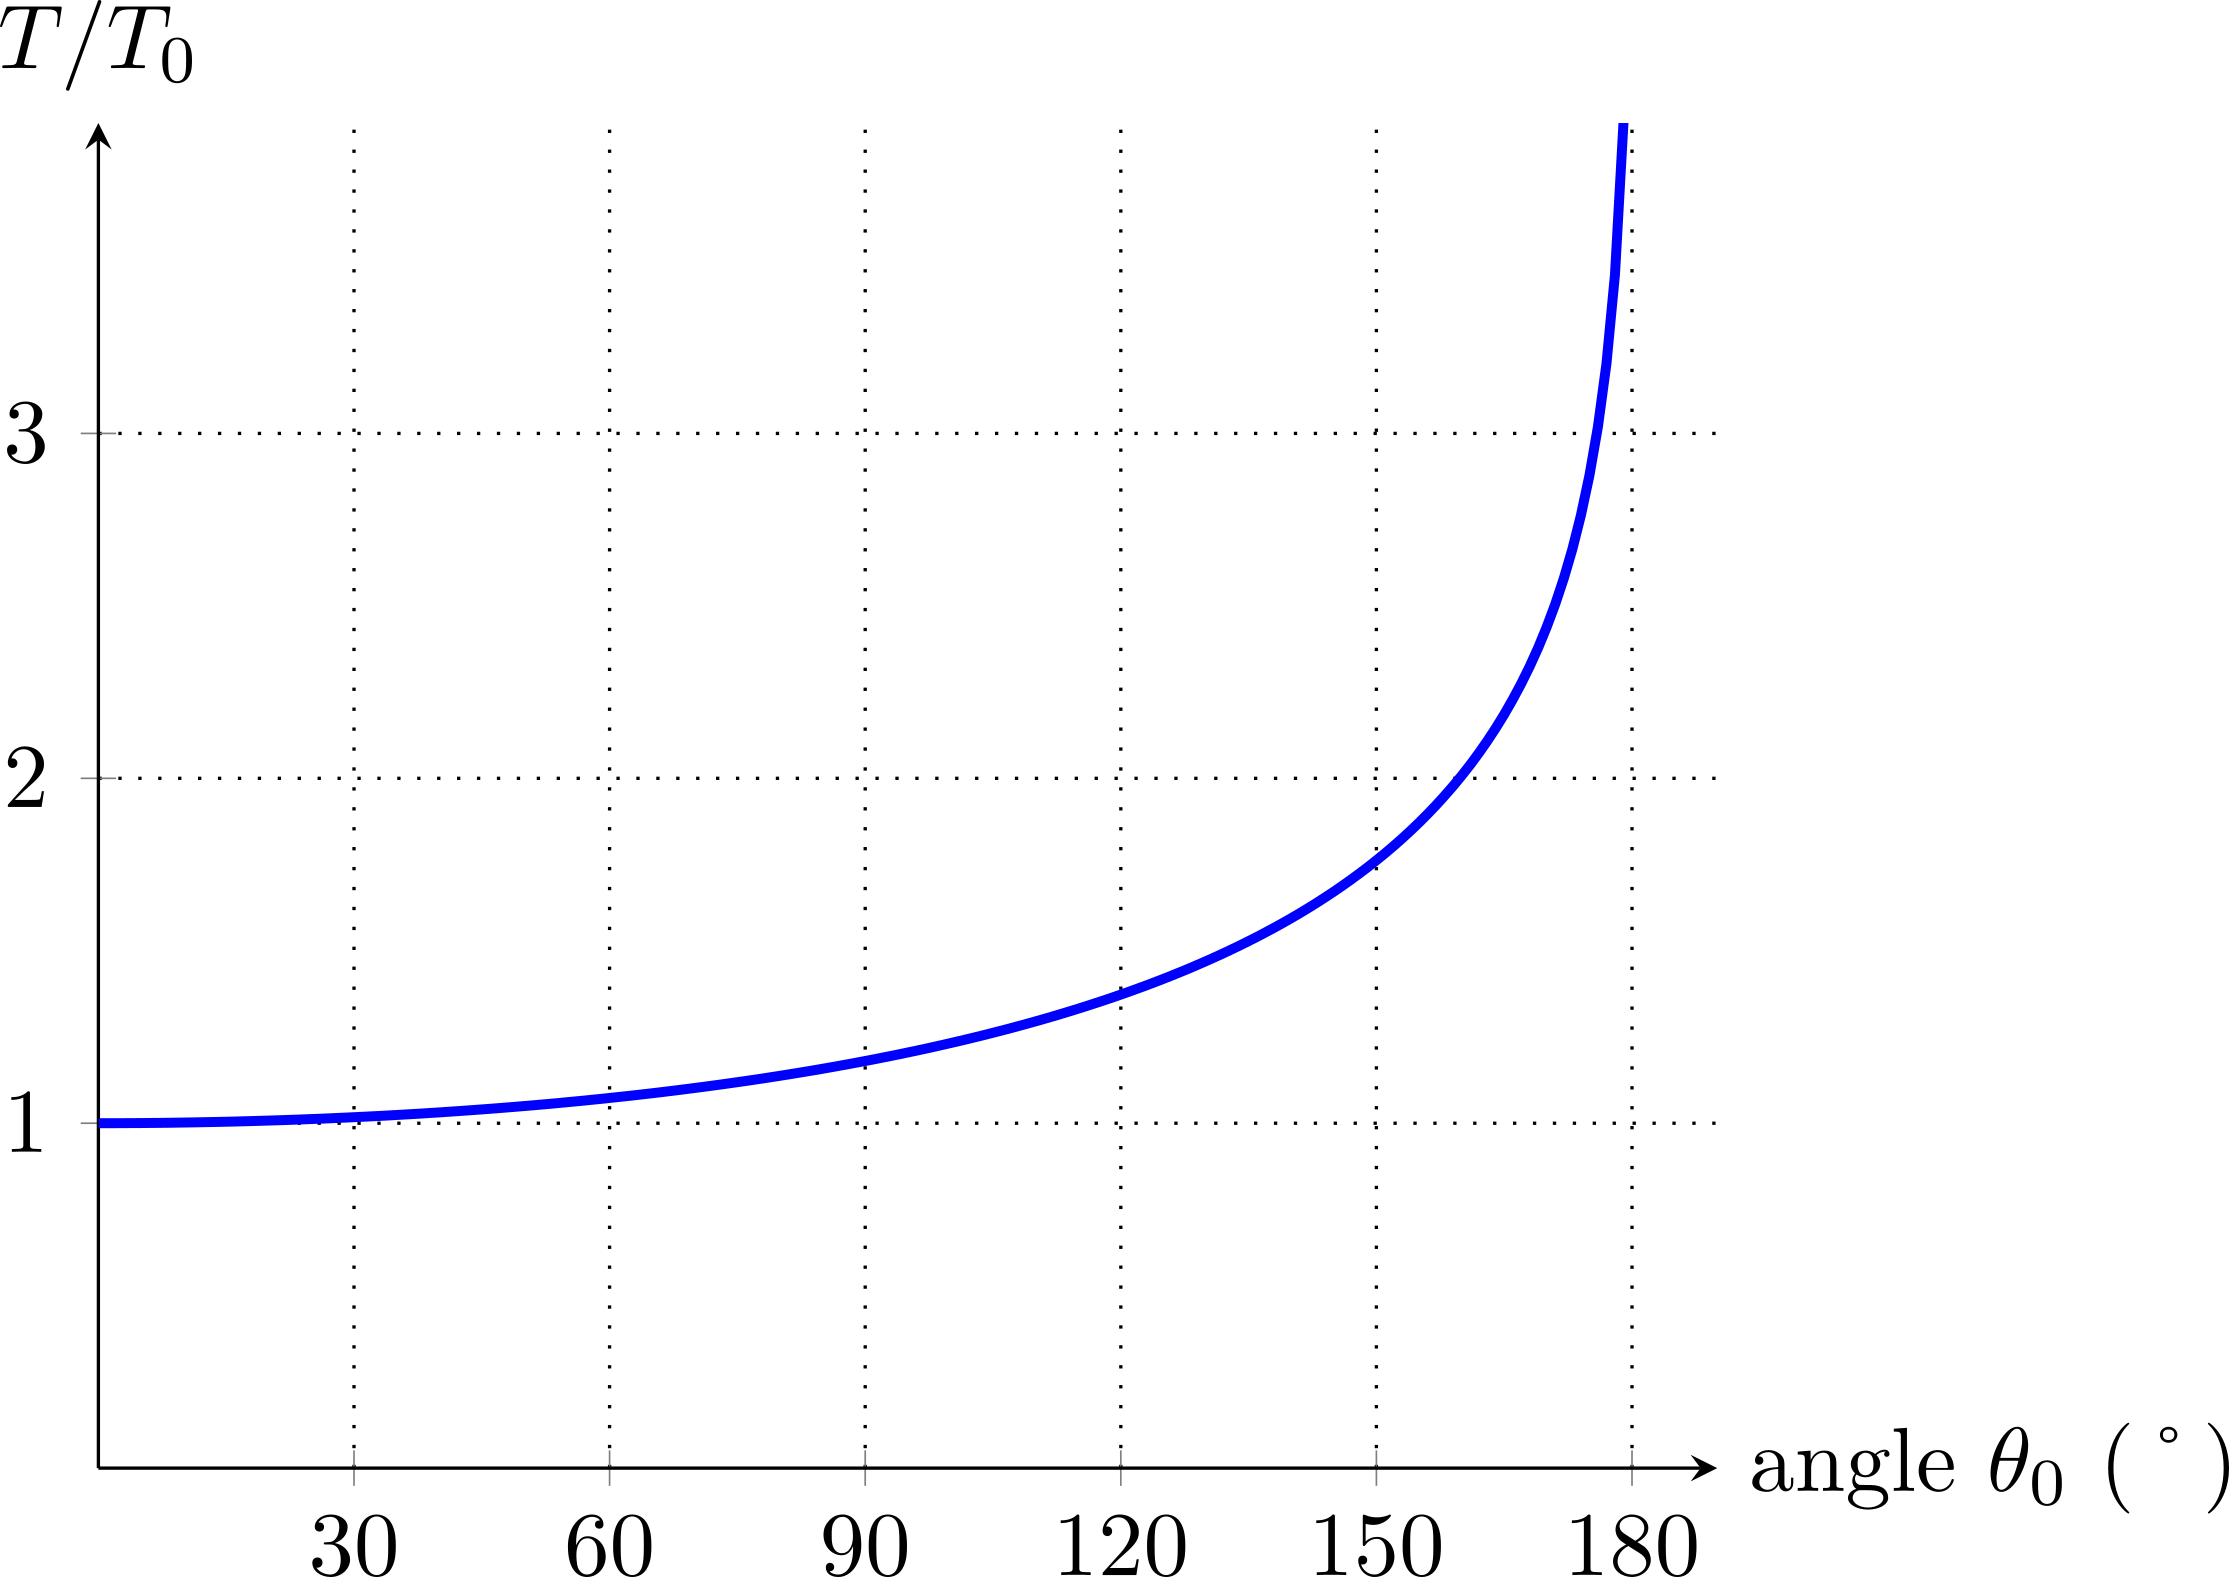
\includegraphics[width=\linewidth]{pendule_gdang}
	\end{center}
\end{minipage}

\begin{tcb*}(appl)<lftt>{Mesure de $g$ par un pendule}
	Ainsi, avec un fil de longueur $\ell = \SI{0.84\pm0.06}{cm}$, on mesure une
	période de $T_0 = \SI{1.84\pm0.1}{s}$. \smallbreak
	\leftcenters{D'où}{$\boxed{g = \SI{9.75}{m.s^{-2}}}$}
\end{tcb*}

\begin{tcb}*(expe)<itc>"trans"{Transition}
	S'il existe de nombreux mouvements plans, il est nécessaire de pouvoir
	décrire des mouvements de rotation qui ne restent pas dans un plan mais
	évoluent dans l'espace 3D.
\end{tcb}

\section{Mouvement courbe dans l'espace}
\subsection{Coordonnées cylindriques}

La manière la plus simple de passer du plan à l'espace est de prendre les
coordonnées polaires et d'y ajouter la coordonnée cartésienne $z$~: on définit
ainsi les coordonnées \textbf{cylindriques}.

\begin{tcb*}(defi){Repère cylindrique et vecteur position}
	\begin{minipage}{0.70\linewidth}
		Le repère cylindrique est constitué d'une origine O autour de laquelle sont
		définis trois vecteurs, $(\ur,\ut,\uz)$, avec $(\ur,\ut)$ la base polaire et
		$\uz$ le vecteur de base cartésienne tel que $\ur \wedge \ut = \uz$. En
		appelant H le projeté orthogonal de M sur le plan polaire, on a
		\[
			\boxed{\OM = \vec{\rm OH} + \vec{\rm HM} = r\ur + z\uz}
			\qet
			\boxed{\norm{\OM} = \sqrt{r^2 + z^2}}
		\]
	\end{minipage}
	\hfill
	\begin{minipage}{0.25\linewidth}
		\begin{center}
			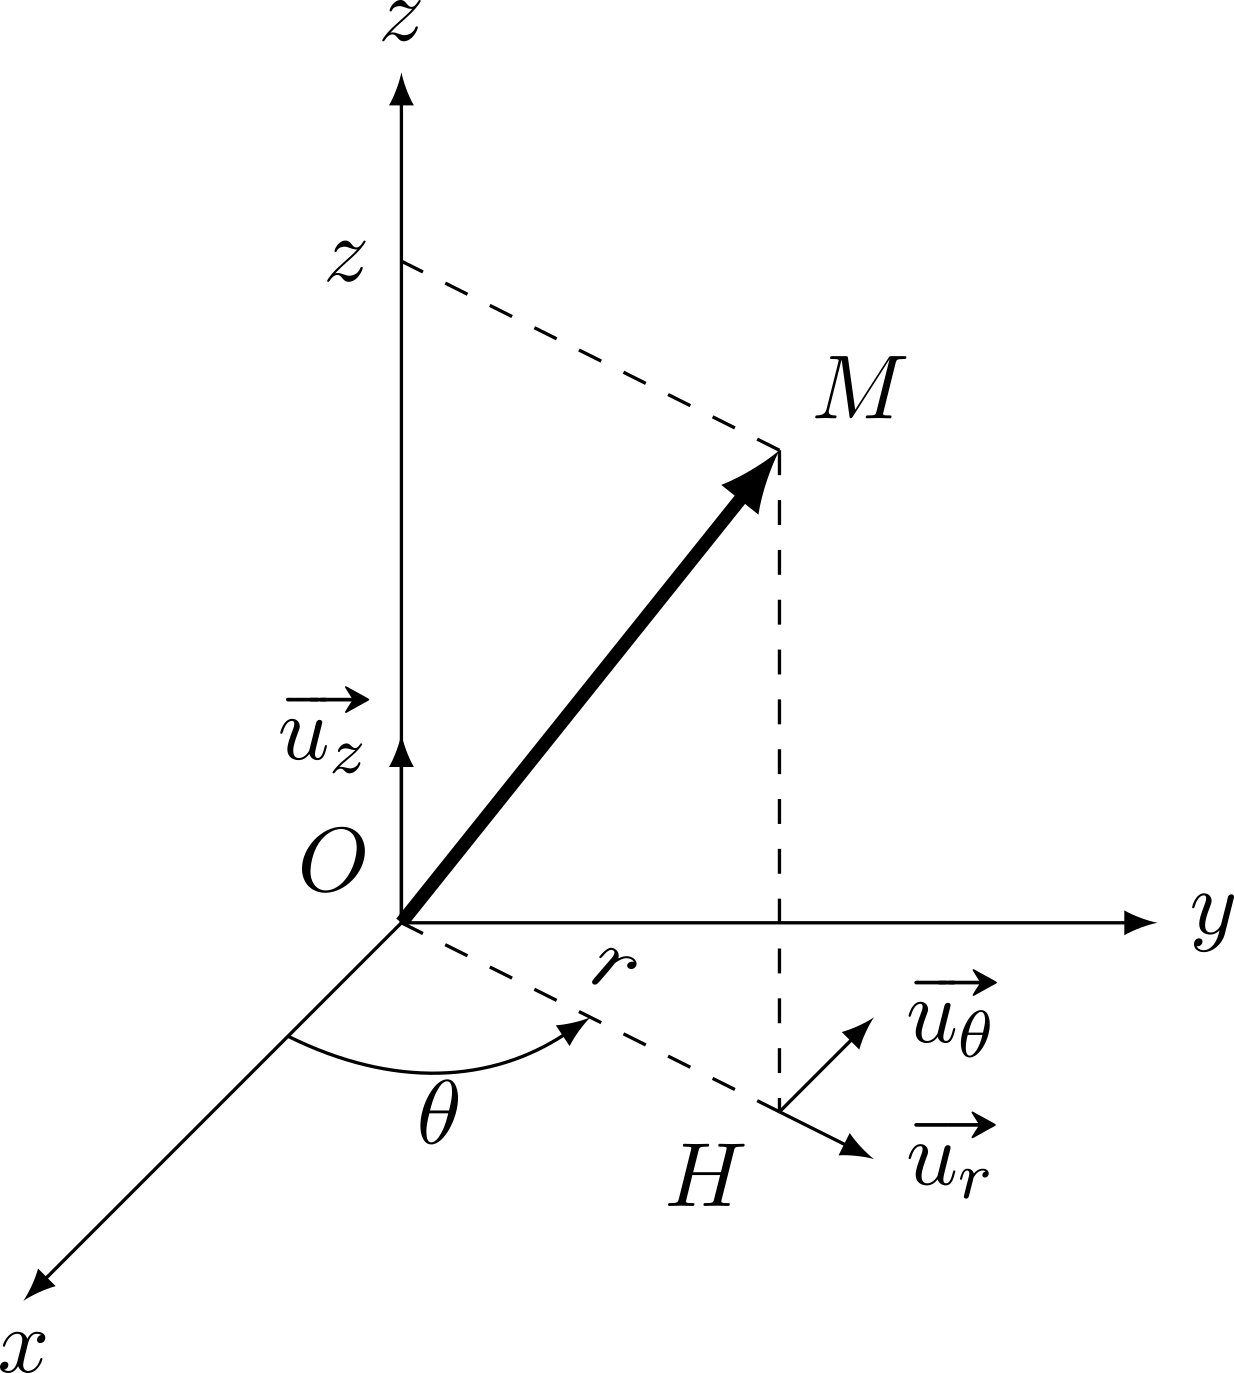
\includegraphics[width=\linewidth]{cyl_rep}
		\end{center}
	\end{minipage}
\end{tcb*}

La détermination de la vitesse et de l'accélération est la même qu'en polaires,
il suffit d'ajouter les dérivées de $z$ puisque $\uz$ est fixe dans le temps.
Ainsi,

\begin{tcb*}(ror){Bilan~: coordonnées cylindriques}
	\begin{itemize}
		\item \leftcenters{\textbf{Coordonnées~:}}{$(r,\tt,z)$}
		\item \leftcenters{\textbf{Vecteurs de base~:}}{$(\ur,\ut,\uz)$}
		\item \leftcenters{\textbf{Position~:}}{$\OM = r\ur + z\uz$}
		\item \leftcenters{\textbf{Vitesse~:}}{$\vf = \rp\ur + r\tp\ut + \zp\uz$}
		\item \leftcenters{\textbf{Déplacement élém.~:}}{$\dd\OM =
				      \dd{r}\ur + r\dd{\tt}\ut + \dd{z}\uz$}
		\item \leftcenters{\textbf{Accélération~:}}{$\DS \af = \left( \rpp
				      -r\tp^2 \right)\ur + \left( 2\rp\tp + r\tpp \right)\ut + \zpp\uz$}
	\end{itemize}
\end{tcb*}

\begin{minipage}{0.70\linewidth}
	Le principe du déplacement élémentaire est de pouvoir définir un volume
	infinitésimal suivant une variation infinitésimale des trois coordonnées. En
	effet, pour une petite variation $(\dd{r}, \dd{\tt}, \dd{z})$, on se déplace
	de $\dd{r}$ dans la direction $\ur$, de $\dd{z}$ dans la direction $\uz$ et
	l'arc de cercle formé par la variation d'angle $\dd{\tt}$ est de longueur
	$r\dd{\tt}$. \bigbreak
\end{minipage}
\hfill
\begin{minipage}{0.25\linewidth}
	\begin{center}
		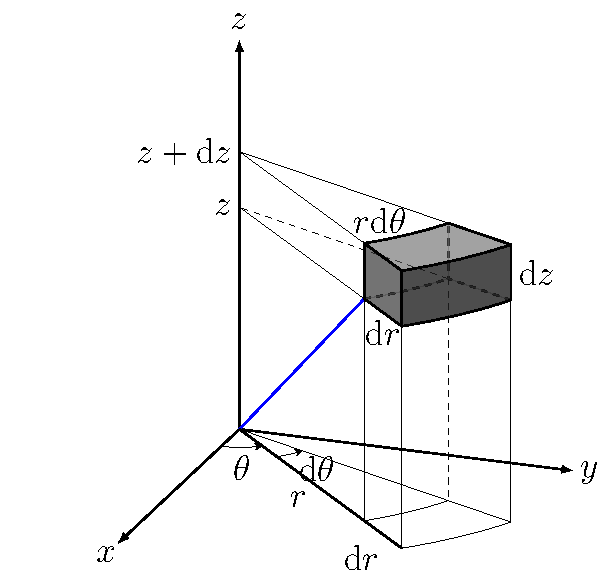
\includegraphics[width=\linewidth]{cyl_vol}
	\end{center}
\end{minipage}

On trouve le volume d'un cylindre de rayon $R$ et de hauteur $h$ en
intégrant sur les trois coordonnées~:
\[V\ind{cyl} = \int_{r'=0}^{R} r'\dd{r'} \int_{\tt'=0}^{2\pi} \dd{\tt'}
	\int_{z'=0}^{h} \dd{z'} = \frac{1}{2}R^2\times 2\pi \times h =
	\boxed{h\pi R^2}\]
C'est l'aire d'un disque multiplié par la hauteur~!

\begin{tcb*}(impo){Choix des coordonnées}
	Dans un problème de mécanique, on choisit les coordonnées judicieusement en
	fonction des symétries du système. \textbf{Sauf proposition de l'énoncé}, on
	utilisera les coordonnées \textbf{cylindriques} pour les mouvements de
	\textbf{rotation}. On utilisera les coordonnées cartésiennes sinon.
\end{tcb*}

\subsection{Coordonnées sphériques}
La manière la plus complète de décrire un mouvement général dans l'espace repose
sur un dernier système de coordonnées, les coordonnées \textbf{sphériques}.

\begin{tcb*}(defi){Repère sphérique}
	\begin{minipage}{0.70\linewidth}
		Le repère sphérique est constitué d'une origine O autour de laquelle sont
		définis trois vecteurs, $(\ur, \ut, \uf)$, tels que
		\[\boxed{\OM = r\ur}
			\qavec
			\boxed{\tt = \widehat{(\uz,\OM)}}
			\qet
			\boxed{\f = \widehat{(\ux,\vec{\rm OP})}}
		\]
		où $\widehat{(\cdot, \cdot)}$ est l'\textbf{angle orienté}, et P le projeté
		orthogonal de M sur le plan polaire. \textbf{$\mathbf{\f}$ correspond à
			$\tt$ des coordonnées polaires.} \bigbreak
	\end{minipage}
	\hfill
	\begin{minipage}{0.25\linewidth}
		\begin{center}
			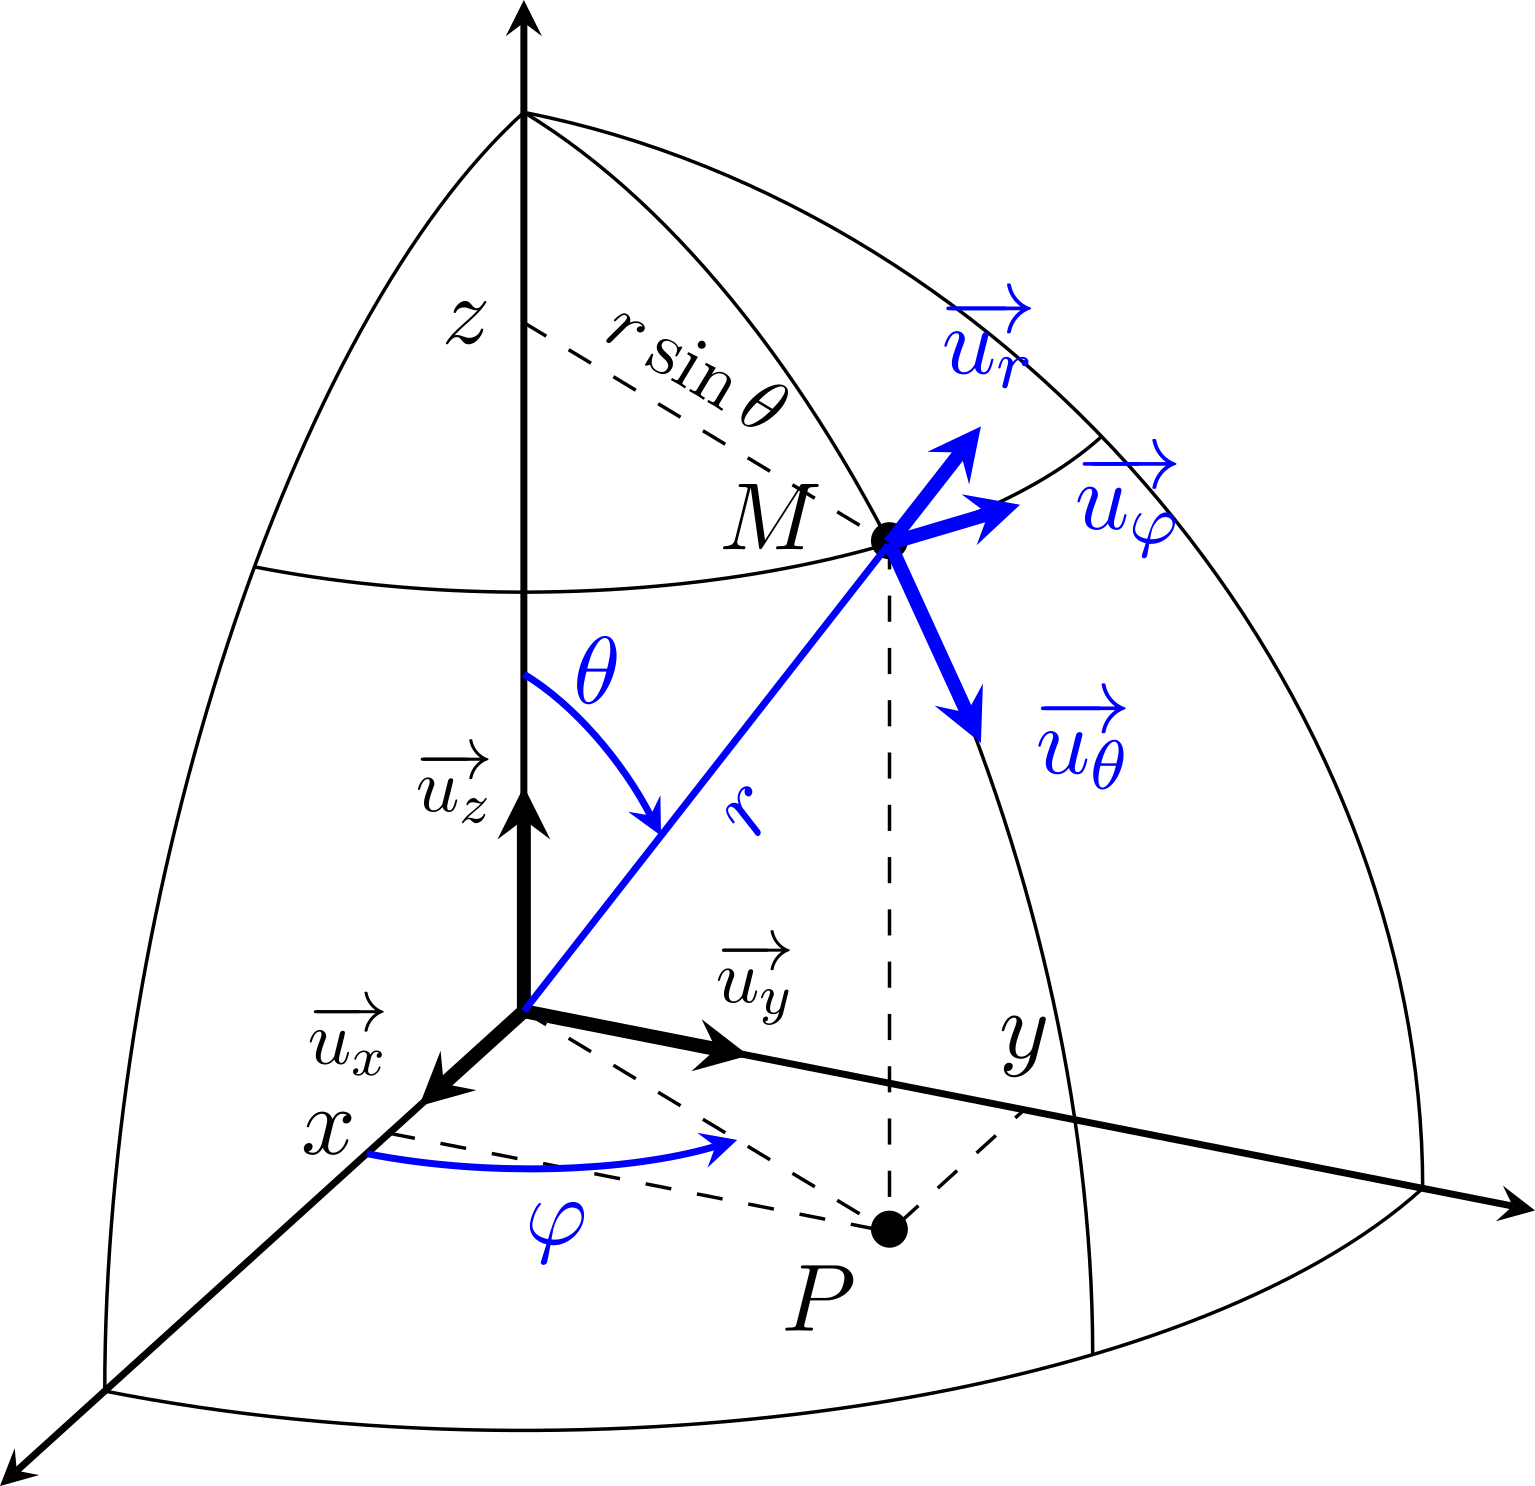
\includegraphics[width=\linewidth]{sph_rep}
		\end{center}
	\end{minipage}
	\begin{itemize}
		\item $\tt \in [0~;~\pi]$ est nommé \textbf{colatitude} ($\lb =
		      \abs{\pi/2 - \tt}$ la latitude)~, et respecte
		      \[  \tan\tt
			      = \frac{\rm OH}{z}
			      \Lra \tt
			      = \atan(\frac{\sqrt{x^2 + y^2}}{z})\]
		\item $\f \in [0~;~2\pi]$ est nommé \textbf{longitude}, et respecte $\DS
			      \f = \atan(\frac{y}{x})$.
	\end{itemize}
\end{tcb*}

\begin{itemize}
	\item Une courbe $\tt = \cte$ est appelée \textbf{parallèle}~; le
	      \textbf{rayon} d'un parallèle est \fbox{$r\sin\tt$}.
	\item Une courbe $\f = \cte$ est appelée \textbf{méridien}~; le
	      \textbf{rayon} d'un méridien est \fbox{$r$}.
\end{itemize}

On peut inverser les définitions en prenant $x = {\rm OP}\cos\f$ et $y = {\rm
	OP}\sin\f$, pour avoir
\[
	\boxed{x = r\sin\tt\cos\f}
	\quad,\quad
	\boxed{y = r\sin\tt\sin\f}
	\qet
	\boxed{z = r\cos\tt}
\]

\begin{tcb*}(exem)<lftt>{Repérage sphérique sur Terre}
	\begin{minipage}{0.70\linewidth}
		Le repérage sur la Terre utilise la latitude et la longitude. Par
		exemple, le lycée \textsc{Pothier} se situe à \ang{47.90}N,
		\ang{1.90;;}E~; on a donc
		\[
			\tt\ind{\textsc{Pothier}} = \ang{42.1}
			\qet
			\f\ind{\textsc{Pothier}} = \ang{1.90}
		\]
	\end{minipage}
	\hfill
	\begin{minipage}{0.25\linewidth}
		\begin{center}
			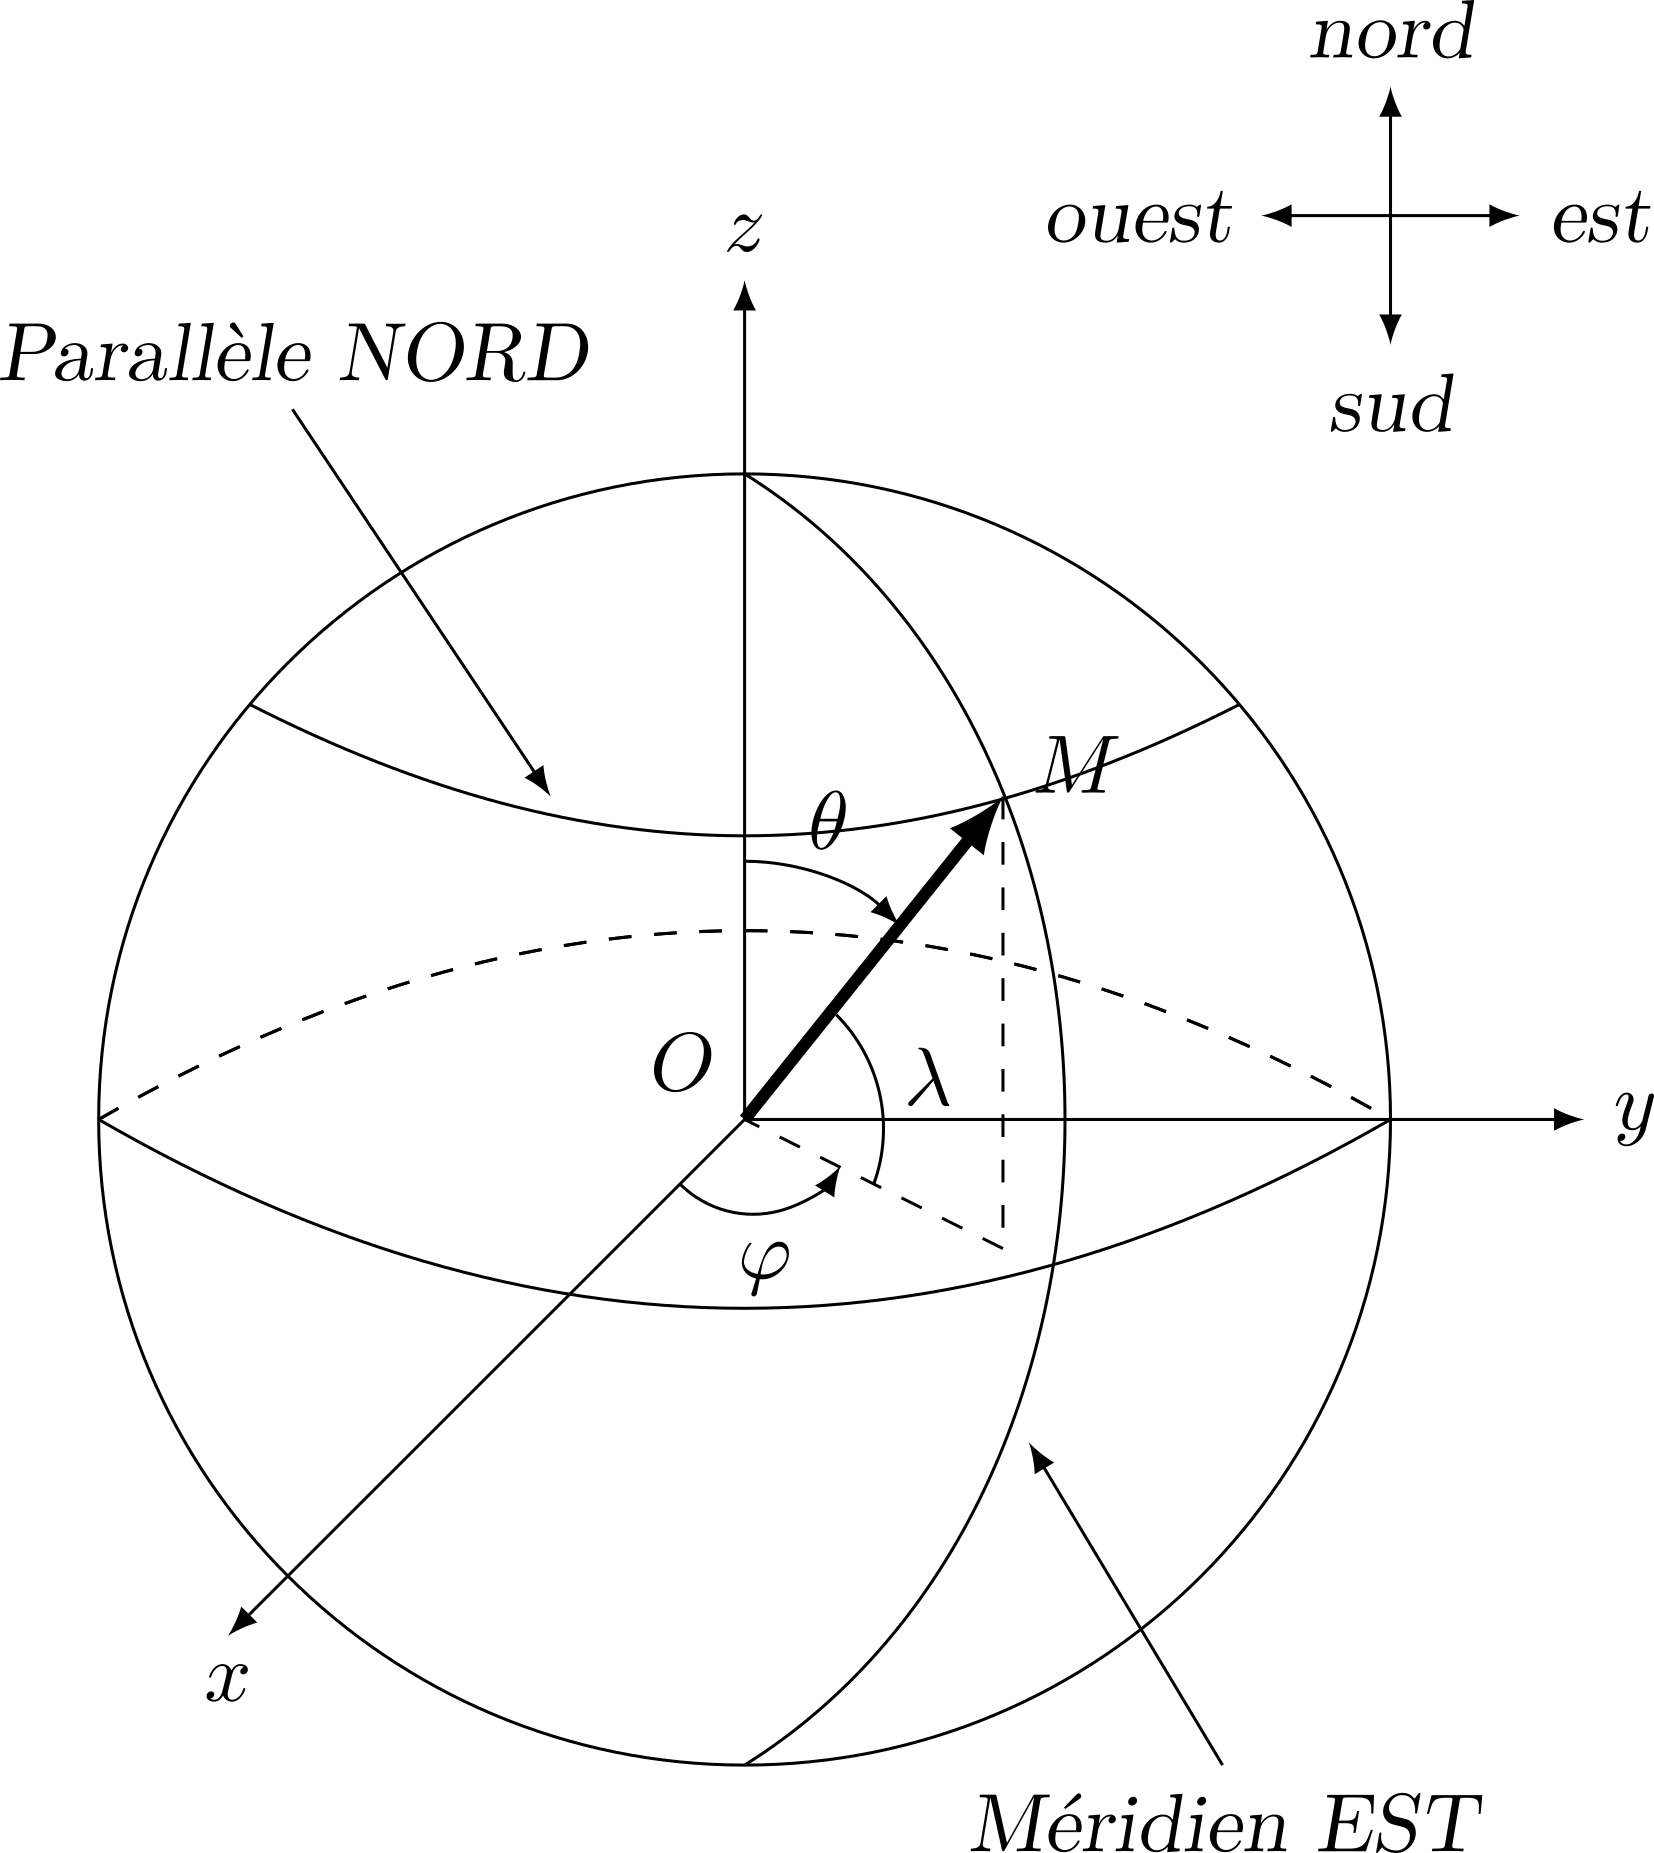
\includegraphics[width=\linewidth]{sph_terre}
		\end{center}
	\end{minipage}
\end{tcb*}


\begin{tcb*}(prop){Déplacement élémentaire sphérique}
	\begin{minipage}{0.70\linewidth}
		\begin{itemize}
			\item Une variation de $\dd{r}$ implique un déplacement de $\dd{r}\ur$~;
			\item Une variation de $\dd{\tt}$ implique un déplacement de
			      $r\dd{\tt}\ut$~;
			\item Une variation de $\dd{\f}$ implique un déplacement de
			      $r\sin\tt\dd{\f}\uf$.
		\end{itemize} \bigbreak
		\[\boxed{\dd\OM = \dd{r}\ur + r\dd{\tt}\ut + r\sin\tt\dd{\f}\uf}\]
	\end{minipage}
	\hfill
	\begin{minipage}{0.29\linewidth}
		\begin{center}
			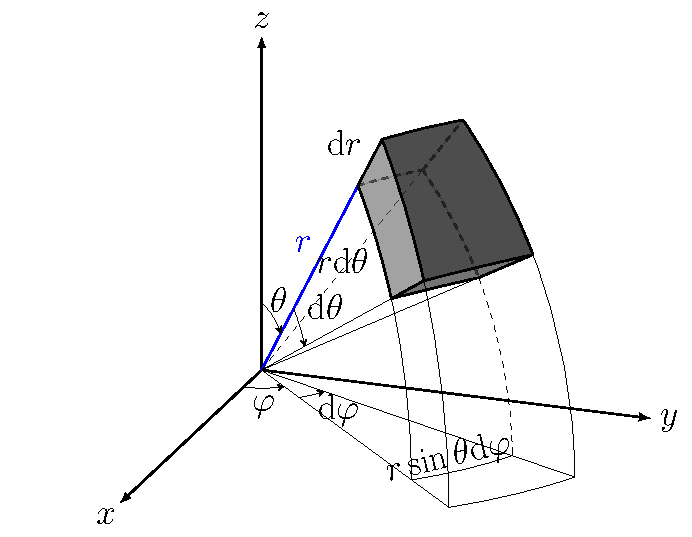
\includegraphics[width=\linewidth]{sph_vol}
		\end{center}
	\end{minipage}
\end{tcb*}

\[V\ind{boule}
	= \int_{r'=0}^{R} r'^2\dd{r'}
	\int_{\tt' = 0}^{\pi} \sin\tt'\dd{\tt'}
	\int_{\f'=0}^{2\pi} \dd{\f}
	= \int_{r'=0}^{R} 4\pi r'^2 \dd{r}
	= \boxed{\frac{4}{3}\pi R^3}
\]

\end{document}
